\documentclass[12pt]{article}
\newcommand{\bottomMargin}{2cm}

\input{structure.tex}

\begin{document}

\renewcommand{\tl}{$0.75$ сек.}
\renewcommand{\ml}{$256$ MB}

\problem{Задача AB21. Кактус}
\addauthor{Автор: Емил Инджев}{2025}{03}{09}

\renewcommand{\header}{
    XLI НАЦИОНАЛНА ОЛИМПИАДА ПО ИНФОРМАТИКА\\
    Национален кръг\\
    Велико Търново, 7 - 10 март 2025 г.\\
    Група AB, 9-12 клас, Ден 2
}

\vspace{0.1in}

\textit{Всички много обичаме задачи с кактуси, но за жалост такива има веднъж на десетилетие. Ето Ви и най-новото попълнение към списъка, това за 20-те години на 21-ви век.}

Вашата група е на експедиция в мексиканската пустиня Чиуауа. Често членове на групата се разделят или изгубват. Решили сте в такива случаи изгубеният член да праща димни сигнли описващи околността му, но тъй като в пустинята няма почти нищо отличително, за отправни точки сте се разбрали да се ползват кактусите в околността. Много е важно да се предаде точно структурата на избрания кактус без никакви грешки, за да бъде намерен изгубения ви другар. Също така, тъй като димните сигнали се пращат бавно и трудно, искате схемата за комуникация да е възможно най-ефикасна (т.е. сигналът да е възможно най-къс). Вашата задача е да измислите такава схема за комуникация. Ще трябва да напишете функция, която получава кактус и го кодира като битов низ (който ще бъде пратен като димен сигнал), и функция, която получава този низ и възстановява оригинално дадения кактус.

Обърнете внимание, че кактус наричаме свързан неориентиран граф без примки (ребро от връх до същия връх) и без повтарящи се ребра, в който всяко ребро е част от най-много един цикъл (но връх може е част от множество цикли). Такъв граф с $N$ върха се описва изцяло от ненареденото си множество от ребра, като всяко ребро е ненаредена двойка от върхове (върховете са номерирани от $0$ до $N-1$). Вижте примерния тест за примерен кактус.

\subsection{Детайли по имплементацията}

Вие трябва да имплементирате функциите \verb|encode| и \verb|decode|:

{\footnotesize \verb|std::vector<bool> encode(int n, std::vector<std::pair<int, int>> edges);|}

Тази функция ще бъде извикана $T$ пъти, като всяко извикване представлява независим събтест. На функцията се подават $N$ и множеството от ребра на кактуса. Тя трябва да кодира графа като низ от битове, който да върне.

Гарантирано е, че редът на ребрата, редът на върховете в дадено ребро и номерацията на върховете са произволно генерирани (но самият кактус може да не е).

{\footnotesize \verb|std::vector<std::pair<int, int>> decode(int n, std::vector<bool> data);|}

Тази функция също ще бъде извикана $T$ пъти, отговарящи на $T$-те извиквания на \verb|encode|. Подават се $N$ и битовия низ, който функцията \verb|encode| е върнала. Тогава \verb|decode| трябва да върне ребрата на кактуса. Забележете, че редът им не е от значение. Също така, не е от значение и редът на върховете в дадено ребро. Важно е обаче върховете да имат същата номерация.

Вашата програма трябва да включва хедър файла \verb|cactus.h|, не трябва да има \verb|main| функция и не трябва да чете от стандартния вход или да пише на стандартния изход.

На оценяващата система, функцията \verb|encode| ще се извиква в един процес, а функцията \verb|decode| в друг, т.е. двете функции не могат да си предават информация по никакъв начин освен чрез върнатия битов низ.

\subsection{Ограничения}

\vspace{0.1em}

\begin{itemize}
\item $ N = 16000 $
\item $ T = 5 $
\end{itemize}

\subsection{Локално тестване}

Предоставени са Ви хедър файл и локален грейдър, които да компилирате с програмата си. Локалния грейдър не използва отделни процеси, т.е. внимавайте да не споделяте глобална информация без да искате (това няма да работи на оценяващата система). Въвежда се първо $T$, последвано от вход за $T$ събтеста. За даден събтест се въвеждат първо $N$ и $M$ (броя ребра), последани от $M$ реда от по две числа, описващи ребрата на графа. Програмата ще изведе броя битове използван на всеки от събтестовете или съобщение за грешка при проблем.

\subsection{Оценяване}

Резултатът Ви за задачата (частта от пълните точки, която ще получите) е равен на минималния Ви резултат сред всички събтестове на всички тестове. Резултат Ви $S$ на даден събтест е 0 при грешен отговор. Иначе зависи от дължината $B$ на битовия низ, който е върнала функцията \verb|encode|. Нека дефинираме:

\begin{itemize}
\item $ T_1 = 240000 $
\item $ T_2 = 256000 $
\item $ T_3 = 272000 $
\item $ T_4 = 304000 $
\item $ T_5 = 400000 $
\end{itemize}

Тогава резултатът Ви е:

\begin{itemize}
\item $ S = 1 $, ако $ B \leq T_1 $
\item $ S = 1 - 0.24 \times \frac{B - T_1}{T_2 - T_1} $, ако $ T_1 \leq B \leq T_2 $
\item $ S = 0.76 - 0.16 \times \frac{B - T_2}{T_3 - T_2} $, ако $ T_2 \leq B \leq T_3 $
\item $ S = 0.60 - 0.16 \times \frac{B - T_3}{T_4 - T_3} $, ако $ T_3 \leq B \leq T_4 $
\item $ S = 0.44 - 0.30 \times \frac{B - T_4}{T_5 - T_4} $, ако $ T_4 \leq B \leq T_5 $
\item $ S = 0.14 \times \frac{T_5}{B} $, ако $ T_5 \leq B $
\end{itemize}

Дадени са някои примерни стойности на $S$ като функция на $B$:

\begin{table}[H]
\begin{tblr}{|Q[c,m]|Q[c,m]||Q[c,m]|Q[c,m]|}
\hline
$B$ & $S$ & $B$ & $S$ \\
\hline
$240000$ & $100\%$ & $336000$ & $34\%$ \\
\hline
$248000$ & $88\%$ & $352000$ & $29\%$ \\
\hline
$256000$ & $76\%$ & $368000$ & $24\%$ \\
\hline
$272000$ & $60\%$ & $384000$ & $19\%$ \\
\hline
$288000$ & $52\%$ & $400000$ & $14\%$ \\
\hline
$304000$ & $44\%$ & $448000$ & $12.5\%$ \\
\hline
$320000$ & $39\%$ & $672000$ & $8.33\%$ \\
\hline
\end{tblr}
\end{table}


\subsection{Пример}

\begin{table}[H]
\begin{tblr}{|m{3cm}|}
\hline
\textbf{Вход} \\
\hline
\texttt{1\\
11 13\\
0 1\\
1 2\\
2 0\\
1 3\\
3 4\\
4 5\\
5 1\\
2 6\\
6 7\\
7 8\\
8 6\\
2 9\\
9 10} \\
\hline
\end{tblr}
\end{table}

Графът от примера е следният:

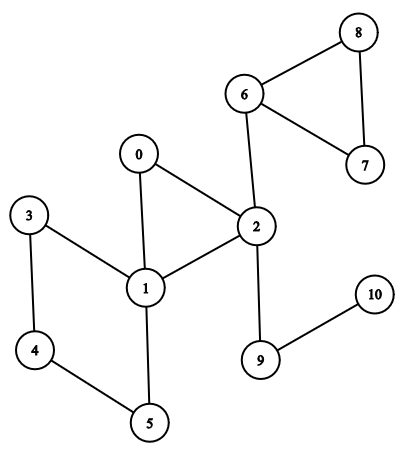
\includegraphics[width=9cm]{./graph.png}

\end{document}
